\documentclass[border=5pt]{standalone}
\usepackage{tikz}
\begin{document}
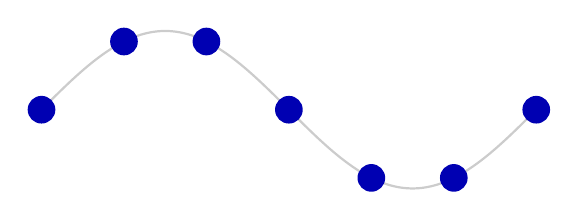
\begin{tikzpicture}
    % faint sine wave for reference
    \draw[gray!40, thick, smooth, samples=100, domain=0:6.2832]
        plot (\x, {sin(\x r)});

    % 7 filled circles arranged along the sine wave
    \foreach \i in {0,...,6} {
        \pgfmathsetmacro{\x}{\i*6.2832/6}      % x from 0 to 2*pi
        \pgfmathsetmacro{\y}{sin(\x r)}         % y = sin(x)
        \fill[blue!70!black] (\x,\y) circle (5pt);
    }
\end{tikzpicture}
\end{document}
